\documentclass[11pt]{article}

\usepackage[margin=1in]{geometry}
\usepackage{amsmath,amssymb}
\usepackage{graphicx}
\usepackage{booktabs}
\usepackage{algorithm}
\usepackage{algpseudocode}
\usepackage[colorlinks=true,linkcolor=blue,citecolor=blue,urlcolor=blue]{hyperref}
\usepackage{natbib}
\usepackage{caption}
\usepackage{subcaption}

\title{Learned Regularization for Robust Image Reconstruction:\\
A Comparative Study of Plug-and-Play Priors under Noise,\\
Undersampling, Model Mismatch, and Distribution Shift}

\author{Your Name\\
\small Affiliation\\
\small \texttt{your.email@example.com}}

\date{\today}

\begin{document}
\maketitle

\begin{abstract}
We study sparse-view computed tomography as a linear inverse problem
and compare classical variational regularization against a learned
image prior integrated into an optimization-based reconstruction
framework. Specifically, we train a noise-level-conditioned CNN
denoiser and use it as an implicit prior inside a Plug-and-Play
proximal-gradient (PnP-PGD) scheme, benchmarking it against filtered
back-projection, Tikhonov (L2), and total variation (TV) regularization.
Using a controlled evaluation protocol -- disjoint train/validation/test
splits, per-condition hyperparameter tuning, and paired statistical
testing -- we find that the learned prior improves PSNR by up to
4\,dB over TV under high measurement noise or severe angular
undersampling, but underperforms TV in the near noise-free regime.
A convergence study reveals that PnP-PGD does not converge to a fixed
point that is simultaneously data-consistent and maximally accurate:
reconstruction quality peaks after a handful of iterations and then
degrades, while the data-fidelity residual continues to rise. We
further show that the learned prior's advantage narrows under
forward-model mismatch (misspecified projection angles) and reverses
under train-test distribution shift, where the prior hallucinates
in-distribution structure on out-of-distribution inputs. We discuss
these findings in light of known instability results for learned
reconstruction methods and argue that robustness evaluation should be
a standard, not optional, component of learned-prior reconstruction
studies.
\end{abstract}

\section{Introduction}
\label{sec:intro}

Image reconstruction from indirect, noisy, and incomplete measurements
is a classical ill-posed inverse problem, arising in computed
tomography (CT), magnetic resonance imaging, and many other imaging
modalities. Given a forward operator $A$ and noisy measurements
\begin{equation}
y = Ax + n,
\end{equation}
the goal is to recover $x$ from $y$ when $A$ is ill-conditioned or
rank-deficient, as is the case for sparse-view CT with few projection
angles. Classical approaches address ill-posedness through explicit
regularization, solving
\begin{equation}
\hat{x} = \arg\min_x \; \tfrac{1}{2}\lVert Ax - y \rVert_2^2 + \lambda R(x),
\end{equation}
with $R$ a hand-crafted prior such as Tikhonov (L2) or total variation
(TV) penalties. In recent years, learned image priors -- most notably
through Plug-and-Play (PnP) methods and deep unrolling -- have been
proposed to replace or augment hand-crafted regularizers with a
denoising neural network, exploiting the empirical observation that
image denoisers implicitly encode rich natural-image statistics
\citep{venkatakrishnan2013plugandplay}.

While learned priors frequently outperform classical regularization on
in-distribution benchmarks, a growing body of work has raised concerns
about their \emph{robustness}: sensitivity to distribution shift, lack
of convergence guarantees, and instabilities under small perturbations
of the input or forward model \citep{antun2020instabilities}. Many
project-level or introductory studies of learned reconstruction report
only in-distribution accuracy, leaving these robustness questions
unaddressed.

This paper documents a controlled, small-scale study designed
explicitly to probe these questions. We deliberately restrict scope
to a simple, cheaply reproducible setting -- sparse-view tomography of
$28\times28$ MNIST-derived images -- in order to run a thorough grid
of experiments with proper train/validation/test protocol rather than
a single headline comparison. Our contributions are:

\begin{itemize}
\item A from-scratch implementation of a sparse-view Radon operator
with exact adjoint, classical regularization baselines (FBP, Tikhonov,
TV-ADMM), and a PnP-PGD solver using a noise-conditioned DnCNN prior.
\item A systematic comparison of PSNR/SSIM accuracy across measurement
noise levels and numbers of projection angles, with validation-tuned
hyperparameters and paired significance testing.
\item A convergence analysis explaining why PnP-PGD selects very few
iterations under validation tuning, showing a peak-then-decay pattern
in reconstruction accuracy that is not visible from residual curves
alone.
\item Two robustness studies -- forward-model mismatch (angle offset
and jitter) and train-test distribution shift (Fashion-MNIST, EMNIST,
and a CT phantom) -- run with hyperparameters frozen at their nominal
values, exposing failure modes not visible under in-distribution
evaluation alone.
\end{itemize}

\section{Related Work}
\label{sec:related}

\paragraph{Variational regularization.} Tikhonov regularization and
total variation \citep{rudin1992tv} remain standard baselines for
ill-posed inverse problems due to their convexity, well-understood
convergence properties, and interpretability. TV in particular is a
strong prior for piecewise-constant images, which makes it a
competitive baseline for digit-like data such as MNIST.

\paragraph{Plug-and-Play priors.}
\citet{venkatakrishnan2013plugandplay} introduced the idea of
replacing the proximal operator of a variational regularizer with an
off-the-shelf denoiser inside an ADMM or proximal-gradient iteration.
Subsequent work analyzed convergence conditions for PnP under
assumptions on the denoiser (e.g. non-expansiveness or bounded
Lipschitz constant) \citep{chan2016pnp,ryu2019pnp}; without such
constraints, plain CNN denoisers offer no convergence guarantee, a
point directly relevant to the convergence behavior we observe in
Section~\ref{sec:experiments}.

\paragraph{Learned denoisers.} DnCNN \citep{zhang2017dncnn}
demonstrated that residual CNNs trained for Gaussian denoising across
a range of noise levels generalize well as plug-in priors. We adopt
this noise-conditioning strategy so that a single trained network can
serve across the PnP iteration trajectory, where the effective
denoising strength is a tunable hyperparameter.

\paragraph{Instabilities and robustness.} \citet{antun2020instabilities}
showed that learned reconstruction methods for CT and MRI can be
unstable to small perturbations and structural changes not present in
training data, in some cases more so than classical methods. Related
work on distribution shift in learned inverse problem solvers
\citep{darestani2021shift} similarly finds that accuracy gains from
learned priors can shrink or reverse under shift. Our distribution
shift and forward-model mismatch experiments are a small-scale,
project-level instantiation of this broader concern, and our findings
(Section~\ref{sec:discussion}) are consistent with it.

\section{Methodology}
\label{sec:method}

\subsection{Forward operator}
We construct a sparse-view Radon transform $A \in \mathbb{R}^{m\times n}$
as an explicit dense matrix by applying the discrete Radon transform to
each canonical basis image and stacking the resulting sinogram columns.
This gives an exact adjoint $A^\top$ (rather than an approximate one,
as is common with implicit/fast Radon implementations), which is
important for the PnP gradient step, and allows the reconstruction
operator to be perturbed independently of the data-generating operator
for the mismatch experiments in Section~\ref{sec:experiments}.
Images are $28\times28$; the number of projection angles and, where
relevant, an angular offset or per-angle jitter are configurable.

\subsection{Classical baselines}
\textbf{Filtered back-projection (FBP)} applies the standard ramp
filter and inverse Radon transform. \textbf{Tikhonov regularization}
solves
\begin{equation}
\hat{x} = \arg\min_x \tfrac{1}{2}\lVert Ax-y\rVert_2^2 + \tfrac{\lambda}{2}\lVert x\rVert_2^2
= (A^\top A + \lambda I)^{-1} A^\top y,
\end{equation}
computed in closed form. \textbf{Total variation} solves
\begin{equation}
\hat{x} = \arg\min_x \tfrac{1}{2}\lVert Ax - y\rVert_2^2 + \lambda \, \mathrm{TV}(x)
\end{equation}
via ADMM with an isotropic TV penalty and a finite-difference operator
$D$, splitting $z = Dx$ and applying the standard shrinkage update on
the split variable.

\subsection{Learned prior: PnP proximal gradient}
We train a DnCNN denoiser $D_\sigma$ conditioned on the noise level
$\sigma$ (following the FFDNet-style noise-map input), on clean MNIST
digits corrupted with Gaussian noise $\sigma \sim \mathcal{U}(0,\sigma_{\max})$,
$\sigma_{\max}=0.3$, using residual learning and an $\ell_2$ loss.
A single trained network is then used across all PnP experiments,
with $\sigma_d$ (the denoising strength argument passed at inference)
treated as a tunable hyperparameter distinct from the training
distribution's noise range.

Reconstruction proceeds by proximal-gradient iteration, replacing the
proximal operator of an explicit regularizer with the learned
denoiser:
\begin{equation}
x_{k+1} = D_{\sigma_d}\big(x_k - \eta \, A^\top(Ax_k - y)\big), \qquad
\eta = 1/L(A^\top A),
\end{equation}
where $L(A^\top A)$ is the largest eigenvalue of $A^\top A$, estimated
by power iteration. The iteration is initialized at the FBP
reconstruction. Algorithm~\ref{alg:pnp} summarizes the procedure.

\begin{algorithm}[h]
\caption{PnP proximal gradient (PnP-PGD)}
\label{alg:pnp}
\begin{algorithmic}[1]
\Require measurements $y$, operator $A$, denoiser $D$, strength $\sigma_d$, step $\eta$, iterations $K$
\State $x_0 \gets \text{FBP}(y)$
\For{$k = 0, \dots, K-1$}
  \State $g_k \gets A^\top(Ax_k - y)$
  \State $x_{k+1} \gets D_{\sigma_d}(x_k - \eta \, g_k)$
\EndFor
\State \Return $x_K$
\end{algorithmic}
\end{algorithm}

\subsection{Evaluation protocol}
Data are split into disjoint training, validation, and test subsets.
All hyperparameters -- $\lambda$ for Tikhonov and TV, and
$(\sigma_d, K)$ for PnP -- are selected by grid search maximizing mean
validation PSNR, independently for each experimental condition
(noise level or number of angles) in Experiments~1--2, and then
evaluated once on the disjoint test set. For the robustness
experiments (Section~\ref{sec:experiments}, E3--E4), hyperparameters
are tuned once at a single nominal condition and then \emph{frozen}
across all mismatch/shift conditions, reflecting a realistic
deployment scenario where a reconstruction pipeline is not retuned
for every possible operating condition. We report PSNR and SSIM as
mean with 95\% confidence intervals over test images, and use a
paired Wilcoxon signed-rank test (matched test images and noise
realizations) to assess the significance of PnP vs.\ TV differences.

\section{Experiments}
\label{sec:experiments}

\subsection{E1--E2: In-distribution accuracy under noise and undersampling}
Table~\ref{tab:e1e2} reports test-set PSNR for representative
conditions (20 projection angles, varying measurement noise
$\sigma$; and fixed $\sigma=0.05$, varying number of angles).

\begin{table}[h]
\centering
\caption{Test PSNR (dB) under varying noise and angular undersampling.
Best method per row in bold. PnP--TV column reports the paired
Wilcoxon test outcome.}
\label{tab:e1e2}
\begin{tabular}{lccccc}
\toprule
Condition & FBP & Tikhonov & TV & PnP-DnCNN & PnP $-$ TV \\
\midrule
$\sigma{=}0$, 20 angles     & 24.2 & 28.9 & \textbf{36.0} & 29.6 & $-6.4$ ($p<10^{-30}$) \\
$\sigma{=}0.01$, 20 angles  & 23.1 & 24.1 & 29.0 & 29.1 & $+0.07$ (n.s., $p=0.27$) \\
$\sigma{=}0.05$, 20 angles  & 15.5 & 17.1 & 20.2 & \textbf{24.0} & $+3.85$ ($p<10^{-30}$) \\
$\sigma{=}0.1$, 20 angles   & 10.4 & 14.7 & 16.9 & \textbf{19.9} & $+3.0$ ($p<10^{-30}$) \\
$\sigma{=}0.2$, 20 angles   & 6.6  & 12.9 & 14.3 & \textbf{15.3} & $+1.0$ ($p<10^{-10}$) \\
\midrule
5 angles, $\sigma{=}0.05$  & 9.1  & 14.2 & 15.5 & \textbf{17.7} & $+2.15$ ($p<10^{-25}$) \\
10 angles, $\sigma{=}0.05$ & 12.1 & 15.9 & 18.4 & \textbf{21.4} & $+3.05$ ($p<10^{-30}$) \\
90 angles, $\sigma{=}0.05$ & 20.6 & 20.0 & 24.1 & \textbf{27.1} & $+3.04$ ($p<10^{-30}$) \\
\bottomrule
\end{tabular}
\end{table}

TV is the strongest classical baseline throughout, consistent with
MNIST digits being close to piecewise-constant. The learned prior
overtakes TV as soon as the problem departs from the near
noise-free, moderately-sampled regime, with gains of up to 4\,dB
PSNR and a corresponding SSIM improvement (0.66 to 0.94 at
$\sigma=0.05$, 20 angles; full SSIM table in the project
repository). At $\sigma=0$ the learned prior underperforms TV by
6.4\,dB, and the two are statistically indistinguishable at
$\sigma=0.01$.

\subsection{E5: Why PnP selects few iterations}
Validation tuning consistently selects a small number of PnP
iterations (5--25 depending on condition). Figure~\ref{fig:convergence}
shows PSNR and the data-fidelity residual $\lVert Ax_k - y\rVert$ as a
function of iteration count, for several values of $\sigma_d$, on 50
test images. PSNR rises rapidly and peaks within the first 5--15
iterations, then \emph{decays} to a lower plateau (e.g.\ $\sigma_d=0.1$:
peak $\approx24.0$\,dB near iteration 10, plateau $\approx22.0$\,dB by
iteration 400). Over the same range, the residual does not decrease;
it rises and plateaus, more steeply for larger $\sigma_d$. This
indicates that the iteration does not converge to a fixed point that
is simultaneously data-consistent and maximally accurate: the
denoiser's implicit prior increasingly dominates the data-fidelity
term as iterations progress, without a corresponding gain in
accuracy. Early stopping is therefore not an artifact of a
coarse hyperparameter grid but an active, necessary part of the
regularization.

\begin{figure}[h]
\centering
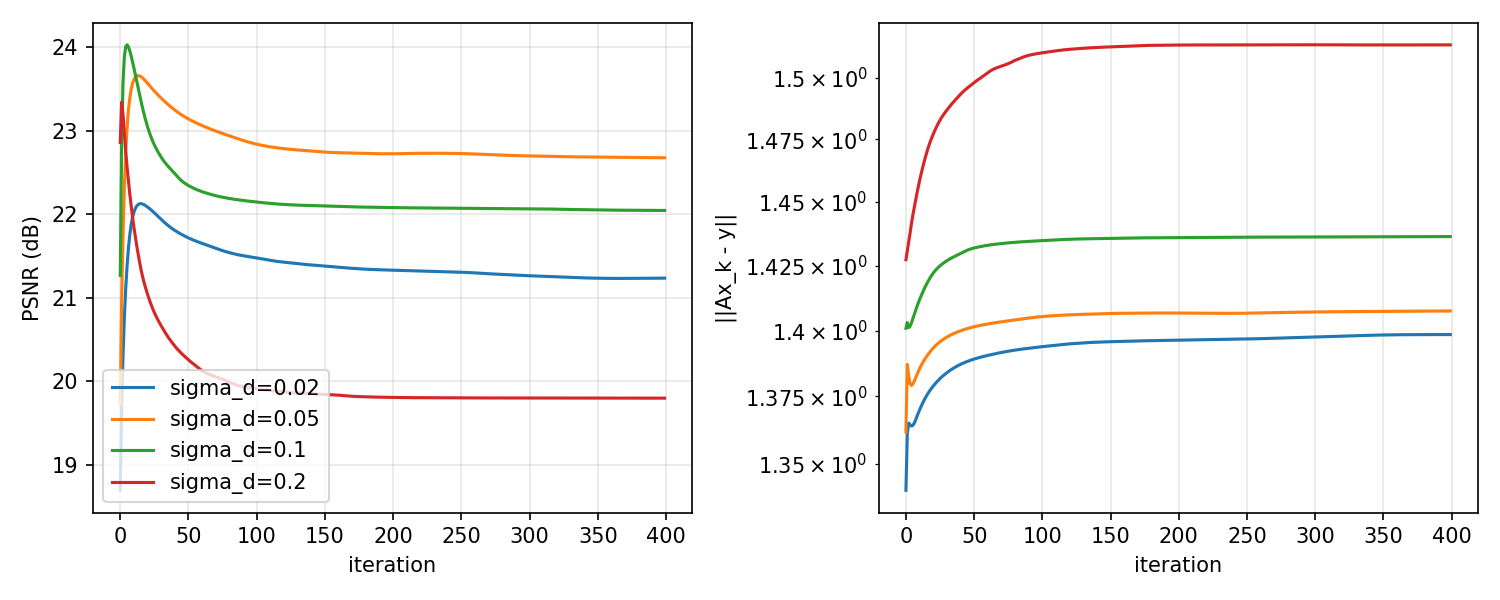
\includegraphics[width=0.95\textwidth]{figures/fig_convergence.png}
\caption{PnP-PGD convergence behavior for several denoising strengths
$\sigma_d$ (50 test images, $\sigma=0.05$, 20 angles). Left: PSNR vs.\
iteration, peaking early then decaying. Right: data-fidelity residual
vs.\ iteration, rising and plateauing rather than decreasing.}
\label{fig:convergence}
\end{figure}

\subsection{E3: Forward-model mismatch}
Measurements are generated with the true 20-angle operator;
reconstruction uses a perturbed operator with either a constant angle
offset (rigid misregistration) or independent per-angle jitter, up to
$4^\circ$, with all hyperparameters frozen at their $\sigma=0.05$,
20-angle values. Table~\ref{tab:e3} summarizes the extremes of the
tested range.

\begin{table}[h]
\centering
\caption{Test PSNR (dB) under forward-model mismatch, hyperparameters
frozen at nominal values.}
\label{tab:e3}
\begin{tabular}{lcccc}
\toprule
Mismatch & TV ($0^\circ \to 4^\circ$) & PnP ($0^\circ \to 4^\circ$) & TV loss & PnP loss \\
\midrule
Constant offset & $20.2 \to 18.6$ & $24.0 \to 20.0$ & $1.6$\,dB & $4.0$\,dB \\
Per-angle jitter & $20.2 \to 19.2$ & $24.0 \to 22.2$ & $1.0$\,dB & $1.8$\,dB \\
\bottomrule
\end{tabular}
\end{table}

PnP remains more accurate than TV in absolute terms throughout the
tested range, but degrades substantially faster in relative terms,
particularly under a constant angular offset. Its advantage over TV
narrows from $+3.85$\,dB at zero mismatch to $+1.48$\,dB at
$4^\circ$ offset.

\subsection{E4: Distribution shift}
The denoiser is trained exclusively on MNIST digits. We evaluate the
full frozen pipeline (nominal $\sigma=0.05$, 20 angles) on
Fashion-MNIST, EMNIST letters, and a resized Shepp-Logan phantom
(single image, 20 independent noise draws). Table~\ref{tab:e4} and
Figure~\ref{fig:shift} summarize the results.

\begin{table}[h]
\centering
\caption{Test PSNR (dB) under train--test distribution shift, frozen pipeline.}
\label{tab:e4}
\begin{tabular}{lcccc}
\toprule
Test set & TV & PnP-DnCNN & PnP $-$ TV \\
\midrule
MNIST (in-distribution)  & 20.3 & \textbf{24.0} & $+3.7$ \\
EMNIST letters (near shift) & 20.1 & \textbf{22.0} & $+1.9$ \\
Fashion-MNIST (far shift) & \textbf{19.6} & 16.5 & $-3.1$ \\
Shepp-Logan phantom (far shift) & \textbf{19.2} & 15.0 & $-4.2$ \\
\bottomrule
\end{tabular}
\end{table}

\begin{figure}[h]
\centering
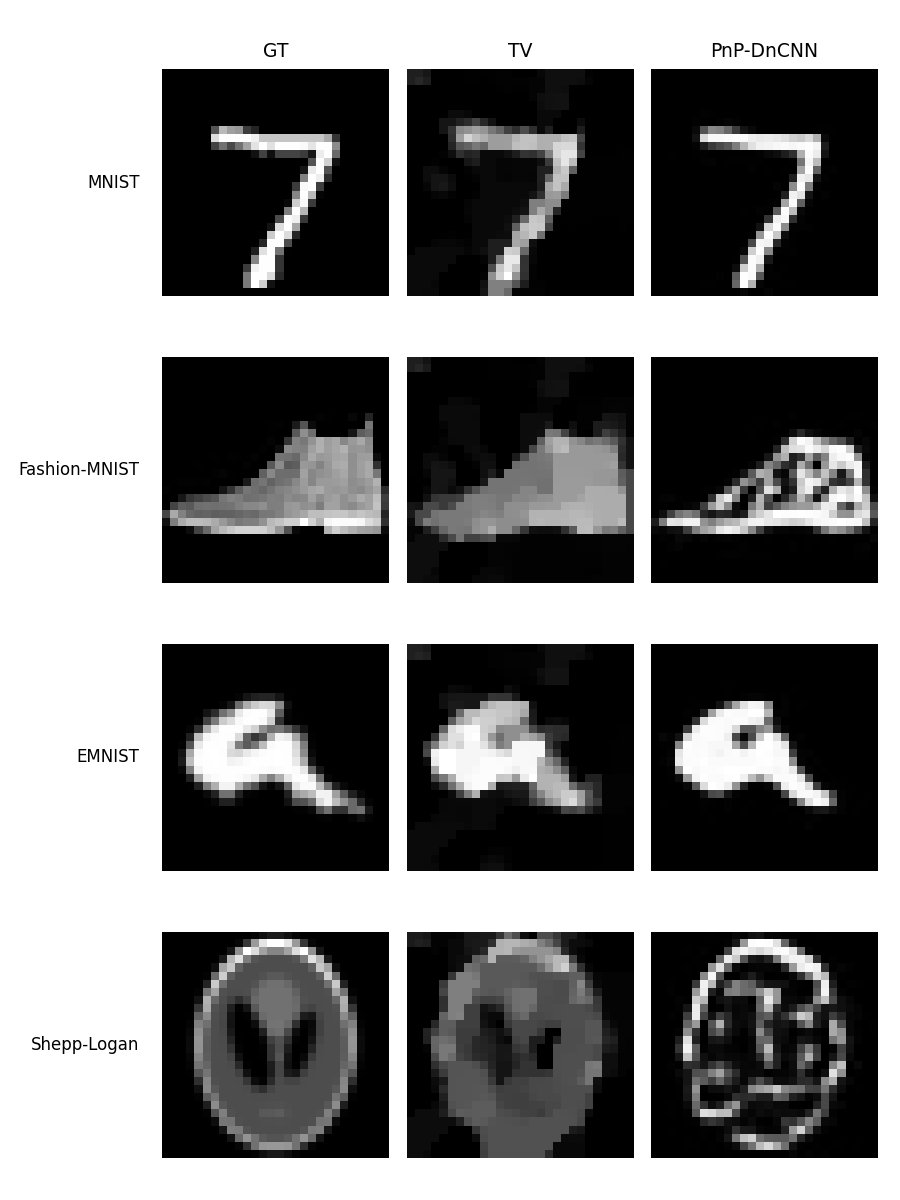
\includegraphics[width=0.85\textwidth]{figures/fig_shift_grid.png}
\caption{Qualitative reconstructions under distribution shift. The
learned prior recovers structure well on MNIST and EMNIST (both
stroke-like), but imposes hallucinated digit/stroke-like structure on
Fashion-MNIST and the CT phantom, both structurally unlike the
training distribution.}
\label{fig:shift}
\end{figure}

The learned prior generalizes to EMNIST letters, which share digits'
stroke-based statistics, but underperforms TV on both far-shift test
sets. Qualitatively (Figure~\ref{fig:shift}), the failure mode is not
generic blur but hallucination: the denoiser imposes plausible-looking
but incorrect digit/stroke-like structure on inputs unlike its
training distribution.

\section{Discussion}
\label{sec:discussion}

Four findings emerge from this study. First, the learned prior's
accuracy advantage over TV is conditional, not universal: it is large
and significant under noise and undersampling, but reverses in the
near noise-free regime, where TV's piecewise-constant assumption is
close to exact for this data. This is a caution against reporting a
single aggregate accuracy number for a learned reconstruction method
without specifying the operating regime.

Second, the convergence study (Section~4.2) shows that PnP-PGD with
an unconstrained CNN denoiser does not behave like a convergent
optimization scheme in the classical sense: accuracy peaks early and
then degrades even as the algorithm continues to iterate, and the
residual does not decrease monotonically. This is consistent with the
theoretical observation that PnP convergence guarantees require
additional constraints on the denoiser (e.g.\ non-expansiveness)
\citep{ryu2019pnp} that plain CNN denoisers, including the one used
here, do not satisfy by construction. In this setting, iteration count
functions as an implicit, and here empirically necessary,
regularization hyperparameter.

Third and fourth, the mismatch and shift experiments show that the
learned prior's advantage is not robust to two distinct kinds of
distribution shift: shift in the forward operator, and shift in the
image distribution. Under forward-model mismatch the learned method
remains more accurate than TV throughout the tested range but loses
its advantage faster; under image distribution shift its advantage
reverses outright, and does so via a qualitatively concerning failure
mode (hallucinated structure) rather than graceful degradation. These
results are consistent with broader findings on instabilities in
learned reconstruction methods \citep{antun2020instabilities} and
support the view that in-distribution accuracy alone is an
insufficient basis for adopting a learned prior in a reconstruction
pipeline; mismatch and shift evaluation should be treated as a
standard part of such studies, not an optional addendum.

\section{Conclusion}
\label{sec:conclusion}

We presented a controlled, small-scale comparison of classical and
learned regularization for sparse-view CT reconstruction, evaluated
under noise, angular undersampling, forward-model mismatch, and
train-test distribution shift. The learned Plug-and-Play prior
substantially outperforms total variation regularization in
ill-posed, noisy regimes, but this advantage is conditional: it
reverses in the near noise-free regime, narrows under forward-model
mismatch, and reverses again under distribution shift, where the
prior hallucinates in-distribution structure. A convergence analysis
further shows that the PnP iteration used here lacks a stable,
accurate fixed point, making early stopping an active regularizer
rather than an implementation detail. Future work could extend this
study to larger, natural-image or clinical-resolution data, provably
convergent PnP variants (e.g.\ with spectrally-normalized or
non-expansive denoisers), and real (rather than simulated) forward
operators.

\section*{Limitations}
This study is intentionally small in scale ($28\times28$ MNIST-derived
images) to allow a thorough experimental grid; trends may not
transfer directly to natural-image or clinical CT resolution and
geometry. The same forward operator is used to generate and
reconstruct data in all experiments except E3 (an ``inverse crime''),
and results reflect a single trained denoiser instance rather than an
average over independent training runs. The PnP scheme used has no
convergence guarantee, and the forward-model mismatch levels tested
(up to $4^\circ$) are moderate; larger or structurally different
mismatches were not evaluated.

\section*{Reproducibility}
Code, trained model, all raw result CSVs, and figures are available
at: \url{https://github.com/YOUR-USERNAME/YOUR-REPO}.

\bibliographystyle{plainnat}
\begin{thebibliography}{9}

\bibitem[Antun et al.(2020)]{antun2020instabilities}
V.~Antun, F.~Renna, C.~Poon, B.~Adcock, and A.~C.~Hansen.
\newblock On instabilities of deep learning in image reconstruction
and the potential costs of AI.
\newblock \emph{Proceedings of the National Academy of Sciences}, 117(48), 2020.

\bibitem[Chan et al.(2016)]{chan2016pnp}
S.~H.~Chan, X.~Wang, and O.~A.~Elgendy.
\newblock Plug-and-play ADMM for image restoration: Fixed-point
convergence and applications.
\newblock \emph{IEEE Transactions on Computational Imaging}, 3(1), 2016.

\bibitem[Darestani et al.(2021)]{darestani2021shift}
M.~Z.~Darestani, A.~S.~Chaudhari, and R.~Heckel.
\newblock Measuring robustness in deep learning based compressive sensing.
\newblock \emph{International Conference on Machine Learning (ICML)}, 2021.

\bibitem[Rudin et al.(1992)]{rudin1992tv}
L.~I.~Rudin, S.~Osher, and E.~Fatemi.
\newblock Nonlinear total variation based noise removal algorithms.
\newblock \emph{Physica D: Nonlinear Phenomena}, 60(1--4), 1992.

\bibitem[Ryu et al.(2019)]{ryu2019pnp}
E.~K.~Ryu, J.~Liu, S.~Wang, X.~Chen, Z.~Wang, and W.~Yin.
\newblock Plug-and-play methods provably converge with properly
trained denoisers.
\newblock \emph{International Conference on Machine Learning (ICML)}, 2019.

\bibitem[Venkatakrishnan et al.(2013)]{venkatakrishnan2013plugandplay}
S.~V.~Venkatakrishnan, C.~A.~Bouman, and B.~Wohlberg.
\newblock Plug-and-play priors for model based reconstruction.
\newblock \emph{IEEE Global Conference on Signal and Information
Processing (GlobalSIP)}, 2013.

\bibitem[Zhang et al.(2017)]{zhang2017dncnn}
K.~Zhang, W.~Zuo, Y.~Chen, D.~Meng, and L.~Zhang.
\newblock Beyond a Gaussian denoiser: Residual learning of deep CNN
for image denoising.
\newblock \emph{IEEE Transactions on Image Processing}, 26(7), 2017.

\end{thebibliography}

\end{document}
